%% This is file AJCEAM-paper.tex is the template file for publications
%% in the "Academic Journal on Computing, Engineering and Applied Mathematics
%% from Universidade Federal do Tocatins, Brazil,
%% https://sistemas.uft.edu.br/periodicos/index.php/AJCEAM/index
%% This file was originally written by Tiago Almeida.
%% First revision: 2019-10-29
%% Second revision:
%%
%% History:
%%           2019-10-29 - First version by Tiago Almeida <tiagoalmeida@uft.edu.br>.
%%           2020-04-09 - English revision by Caio Machado <caio.machado@uft.edu.br>
%%

% Options
%     eng:   English Language
%     por:   Portuguese Language
%     blind: The version for reviewers is compiled (author data is hidden)


\documentclass[eng]{ajceam-class}
%
% Publication Title
\title{Ghostbusters}


% Short title for the header (copy the main title if it is not too long)
\shorttitle{Ghostbusters}
       
% Authors
\author[1]{Diana L. Hernández-Almeida}
\author[1]{José A. López-Torres}
\author[1]{Axel D. Luna-Hernández}
\author[1]{Jorge E. Nevarez-Soto}

% Author Affiliations
\affil[1]{Tecnologico de Monterrey}

% Surname of the first author of the manuscript
%\firstauthor{Hernández, López, Luna and Nevarez}

%Contact Author Information
%\contactauthor{Name A. Surname}           % Name and surname of the contact author
%\email{name.surname@email.com}            % Contact Author Email

% Publication data (will be defined in the edition)
%\thisvolume{XX}
%\thisnumber{XX}

\thismonth{Septiembre}
\thisyear{2025}

% Place your particular definitions here
\newcommand{\vect}[1]{\mathbf{#1}}  % vectors

% Insert here the abstract in English language
\abstract{This study addresses the task of classifying narratives of paranormal phenomena shared in online communities. The objective was to implement and evaluate naïve Bayes classifiers on stories collected through web scraping from the platform \textit{Your Ghost Stories}. The dataset comprised 1,828 narratives labeled into two categories: \textit{Haunted} (823) and \textit{Other} (1,005). Preprocessing included tokenization, stop word removal, and the construction of sparse matrices to represent word frequencies, yielding 6,727 unique terms. 
Two baseline implementations of naïve Bayes, using the \texttt{e1071} and \texttt{naivebayes} packages, achieved identical results with an accuracy of 61.6\%, precision of 57.1\%, recall of 50.2\%, and F1-score of 53.4\% for the \textit{Haunted} class. Extending the model with a Poisson distribution improved performance to 69.6\% accuracy and an F1-score of 60.9\%, although it generated warnings due to zero counts. Incorporating Laplace smoothing mitigated these warnings, producing a stable model with 69.2\% accuracy and an F1-score of 60.0\%. Cross-validation identified an optimal Laplace parameter ($\lambda = 0.2$), confirming the trade-off between predictive power and robustness. Overall, the results demonstrate that naïve Bayes can provide meaningful classification of highly subjective paranormal narratives, and that probabilistic extensions such as Poisson modeling and Laplace smoothing substantially enhance performance and stability. 
}

\keywords{naïve Bayes, text mining, web scraping, paranormal phenomena, classification, NLP}


% Start document
\begin{document}

% Include title, authors, abstract, etc.
\maketitle
\thispagestyle{fancy}
%\printcontactdata



% Main body of manuscript
\section{Introducción}
\firstword{E}{n}% Capital letter in first word
internet existen numerosas comunidades en las que las personas comparten experiencias relacionadas con fantasmas, UFOs, brujería, criaturas extrañas y otros sucesos inexplicables. Estas narraciones suelen estar redactadas con descripciones detalladas y un lenguaje subjetivo, lo que dificulta su clasificación sistemática. La diversidad de fenómenos reportados y la ausencia de categorías estandarizadas complican la organización y el análisis de este tipo de contenidos.  

En el campo del procesamiento de lenguaje natural (NLP), los modelos probabilísticos han sido ampliamente utilizados en tareas de clasificación de texto\cite{zhang2004naive, mccallum1998comparison}. Entre ellos, el clasificador \textit{naïve Bayes} ha destacado por su eficacia al trabajar con datos de alta dimensionalidad y representaciones dispersas. A pesar de la fuerte suposición de independencia condicional entre las variables, distintos estudios han demostrado que sigue siendo una línea base competitiva en el ámbito de la clasificación.  

Este estudio aplica un clasificador \textit{naïve Bayes} al análisis de narraciones paranormales recopiladas mediante \textit{web scraping} de la plataforma \textit{Your Ghost Stories}. El conjunto de datos obtenido incluye el título, lugar, tipo de evento y descripción de cada historia. Inicialmente se evaluaron dos implementaciones estándar de \textit{naïve Bayes}, y posteriormente se incorporaron extensiones probabilísticas para enfrentar limitaciones propias de este enfoque. Entre ellas destacan el uso de la distribución Poisson para modelar datos de conteo, la aplicación de suavizamiento de Laplace para manejar la abundancia de ceros y la validación cruzada para la selección óptima de parámetros. De esta forma, el objetivo principal es valorar la capacidad de los modelos \textit{naïve Bayes} y sus variantes para categorizar estas narraciones en clases significativas, resaltando tanto su potencial como las limitaciones al tratar con datos textuales no convencionales y altamente subjetivos.  



\section{Metodología}

La metodología consistió en aplicar técnicas de clasificación supervisada a narrativas textuales, organizadas en cuatro fases principales: recolección de datos, preprocesamiento, representación de los textos en formato matricial y entrenamiento de un clasificador probabilístico.  

La recolección de datos se realizó mediante técnicas de \textit{web scraping}, seleccionando un portal especializado en relatos de fenómenos paranormales. Este procedimiento permitió construir una base a partir de historias reales publicadas por usuarias y usuarios, preservando para cada registro atributos básicos como título, lugar, categoría asignada y descripción narrativa.  

El preprocesamiento incluyó operaciones comunes en análisis de texto, como normalización de caracteres, eliminación de signos de puntuación, filtrado de palabras vacías y tokenización\cite{wickham2023r4ds, wickham2019stringr}. Estas transformaciones convirtieron las narraciones en unidades comparables y facilitaron su posterior análisis cuantitativo.  

Para la representación matemática de los textos se construyó una matriz documento-término, donde cada relato se corresponde con una fila y cada palabra con una columna. Dada la naturaleza de los datos, esta matriz resultó dispersa, lo cual es típico en tareas de minería de texto\cite{wickham2023r4ds, wickham2019stringr}.  

Posteriormente, se entrenaron clasificadores \textit{naïve Bayes} como modelo base, utilizando tanto la implementación estándar de la librería \texttt{e1071} como la del paquete \texttt{naivebayes}\cite{meyer2021e1071} y \texttt{naivebayes} \cite{majka2019naivebayes}.. El desempeño de los modelos se evaluó con métricas estándar en clasificación: exactitud, precisión, recall, puntaje F1 y matriz de confusión.  

Con el fin de superar las limitaciones de las versiones básicas, se implementaron tres extensiones metodológicas. En primer lugar, se incorporó la distribución Poisson para modelar de manera más adecuada los datos de conteo presentes en la matriz dispersa. En segundo lugar, se aplicó el suavizamiento de Laplace como estrategia para manejar la abundancia de ceros y reducir el impacto de frecuencias nulas en la estimación de probabilidades. Finalmente, se utilizó validación cruzada para explorar diferentes valores del parámetro de suavizamiento y seleccionar aquel que maximizara el desempeño del modelo de manera estable.  

Este diseño metodológico permitió evaluar tanto la capacidad base del clasificador \textit{naïve Bayes} como las mejoras derivadas de ajustes probabilísticos específicos para datos textuales.  


\section{Aplicación}

El procedimiento descrito en la metodología se implementó utilizando los relatos obtenidos de la plataforma \textit{Your Ghost Stories}. El conjunto de datos final incluyó 1,828 narraciones, de las cuales 823 se clasificaron como \textit{Haunted} y 1,005 como \textit{Other}. Esta distribución relativamente balanceada permitió entrenar y evaluar modelos de clasificación sin un sesgo severo hacia una sola categoría.  

Como parte del análisis exploratorio, se identificaron las palabras más frecuentes en la base, entre las que destacaron \textit{house}, \textit{time}, \textit{night} y \textit{door}. Estos términos reflejan la recurrencia de contextos domésticos y nocturnos en los relatos paranormales. La Figura~\ref{fig:top20_app} muestra las 20 palabras más comunes después del preprocesamiento.  

\begin{figure}[H]
  \centering
  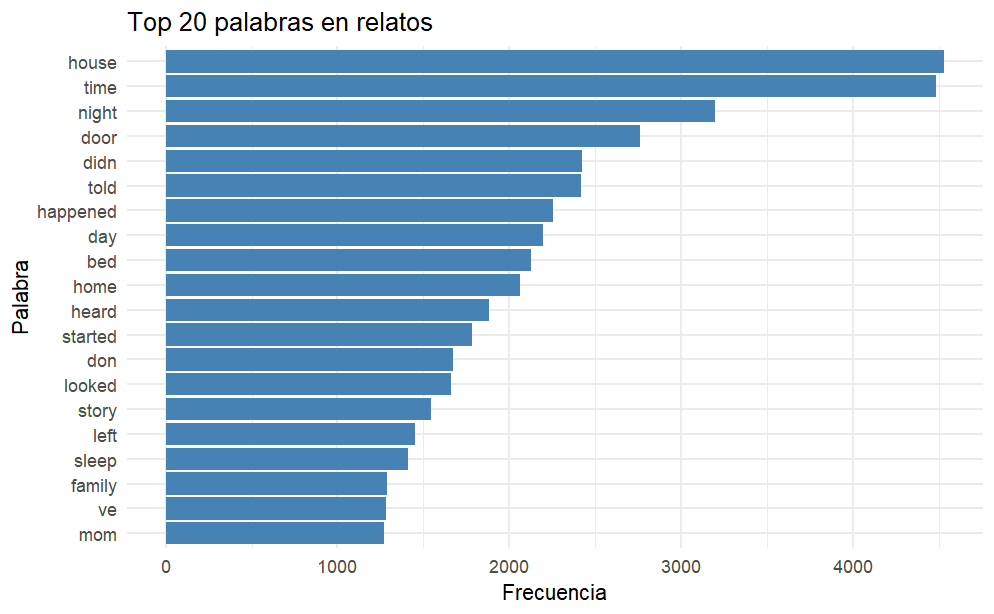
\includegraphics[width=0.85\columnwidth]{top20}
  \caption{Top 20 palabras más frecuentes en los relatos.}
  \label{fig:top20_app}
\end{figure}

En cuanto a la modelación, el problema se redujo a una clasificación binaria entre las categorías \textit{Haunted} y \textit{Other}. El conjunto de datos fue dividido en 70\% para entrenamiento y 30\% para prueba. Se ajustaron dos versiones del clasificador \textit{naïve Bayes}, una con la librería \texttt{e1071} y otra con la librería \texttt{naivebayes}.  

Los resultados se presentan en la Tabla~\ref{tab:comparacion_app}. Ambas implementaciones arrojaron métricas idénticas: una exactitud de 61.6\%, precisión de 57.1\%, recall de 50.2\% y F1 de 53.4\% para la clase \textit{Haunted}. El desempeño moderado indica que el modelo logra capturar ciertos patrones, pero aún tiende a clasificar incorrectamente parte de los relatos de tipo \textit{Haunted}.  

\begin{table}[H]
 \centering
 \caption{Resultados comparativos de las implementaciones estándar del clasificador \textit{naïve Bayes}.}
 \label{tab:comparacion_app}
 {\small
 \begin{tabular}{lcccc}
  \hline
  \hline
  \thead{Modelo} & \thead{Accuracy} & \thead{Precisión} & \thead{Recall} & \thead{F1} \\
  \hline
  e1071::naiveBayes & 0.6157 & 0.5708 & 0.5021 & 0.5342 \\
  naivebayes & 0.6157 & 0.5708 & 0.5021 & 0.5342 \\
  \hline
  \hline
 \end{tabular}}
\end{table}

Un problema que enfrentan estas primeras implementaciones del clasificador \textit{naïve Bayes} es el supuesto de normalidad en los predictores, lo cual resulta poco adecuado cuando los datos corresponden a conteos. Para abordar esta limitación se probó la distribución Poisson como alternativa.  

\begin{table}[H]
 \centering
 \caption{Comparación del modelo estándar frente a la versión Poisson y Poisson con Laplace.}
 \label{tab:comparacion_poisson}
 {\small
 \begin{tabular}{lcccc}
  \hline
  \hline
  \thead{Modelo} & \thead{Accuracy} & \thead{Precisión} & \thead{Recall} & \thead{F1} \\
  \hline
  e1071::naiveBayes & 0.6157 & 0.5708 & 0.5021 & 0.5342 \\
  naivebayes: & 0.6157 & 0.5708 & 0.5021 & 0.5342 \\
  naivebayes::Poisson & 0.6958 & 0.6989 & 0.5394 & 0.6089 \\
  naivebayes::Poisson\_Laplace & 0.6812 & 0.7012 & 0.4772 & 0.5679 \\
  \hline
  \hline
 \end{tabular}}
\end{table}

Los resultados muestran que el modelo con distribución Poisson mejoró considerablemente el desempeño, alcanzando una exactitud de 69.6\% y un F1 de 60.9\%. Sin embargo, esta versión generó múltiples advertencias debido a la abundancia de ceros en la matriz dispersa. Para contrarrestar este problema se aplicó el suavizamiento de Laplace, lo que eliminó los errores pero redujo ligeramente el desempeño (F1 de 56.8\%).  

Finalmente, se aplicó validación cruzada para seleccionar el mejor valor del parámetro de suavizamiento.  

\begin{table}[H]
 \centering
 \caption{Resultados de validación cruzada con diferentes valores de $\lambda$ en el suavizamiento de Laplace.}
 \label{tab:cv_laplace}
 {\small
 \begin{tabular}{lc}
  \hline
  \hline
  \thead{Laplace ($\lambda$)} & \thead{Accuracy promedio} \\
  \hline
  0.1 & 0.6513 \\
  0.2 & 0.6458 \\
  0.3 & 0.6513 \\
  0.4 & 0.6482 \\
  0.5 & 0.6458 \\
  0.6 & 0.6443 \\
  0.7 & 0.6435 \\
  0.8 & 0.6427 \\
  0.9 & 0.6411 \\
  1.0 & 0.6380 \\
  \hline
  \hline
 \end{tabular}}
\end{table}

El valor óptimo identificado fue $\lambda = 0.2$. Aunque este ajuste no alcanzó la misma exactitud del modelo Poisson sin suavizamiento, sí proporcionó un desempeño estable y libre de advertencias. Con este ajuste, el modelo obtuvo una exactitud de 69.2\% y un F1 de 60.0\%, valores lo suficientemente cercanos para considerarse una alternativa robusta frente al problema de los ceros.  


\section{Conclusiones}

El presente estudio evaluó la aplicación de \textit{naïve Bayes} para categorizar relatos de fenómenos paranormales recopilados mediante \textit{web scraping} de la plataforma \textit{Your Ghost Stories}. El análisis demostró que las versiones estándar del clasificador, implementadas con las librerías \texttt{e1071} y \texttt{naivebayes}, alcanzaron un desempeño moderado con una exactitud de 61.6\% y un F1 de 53.4\% para la clase \textit{Haunted}.  

La incorporación de la distribución Poisson permitió mejorar sustancialmente los resultados, logrando una exactitud cercana al 70\% y un F1 de 60.9\%. No obstante, este modelo generó múltiples advertencias debido a la presencia de ceros en la matriz dispersa. Para superar esta limitación se aplicó el suavizamiento de Laplace, que estabilizó el entrenamiento y redujo los errores, aunque con un ligero costo en el desempeño. Mediante validación cruzada se identificó un valor óptimo de $\lambda = 0.2$, el cual ofreció un equilibrio adecuado entre robustez y precisión, con métricas muy cercanas a las del modelo Poisson puro.  

En conjunto, los resultados muestran que los clasificadores \textit{naïve Bayes} constituyen una herramienta viable para el análisis de narraciones textuales altamente subjetivas, y que las extensiones probabilísticas pueden mejorar notablemente su rendimiento. Entre las principales limitaciones se encuentra la dependencia del modelo en supuestos simplificadores y la sensibilidad a la representación de los datos.  

Como líneas futuras de investigación se sugiere explorar técnicas de representación más avanzadas, como embeddings contextuales\cite{scutari2010bnlearn}, así como evaluar clasificadores alternativos capaces de capturar dependencias más complejas en los textos. Estas estrategias podrían complementar los hallazgos aquí presentados y contribuir a un análisis más preciso de fenómenos narrativos no convencionales.  



% Include references
\insertbibliography{References}


\end{document}
